\section{Published layouts and requests available within an expansion}
\label{sec:followup-results}
The earlier results leave two natural questions. Would established placement methods do better than the local heuristic? And does their ranking depend on offering future graph work before its preceding reads finish? The follow-up tests both questions while preserving the original experiments. Its comparisons use the default controller; the previously reported policy and mapper sweeps remain supporting evidence for that controller choice's importance.

\subsection{The cost of restricting future work}
Table~\ref{tab:barriers} shows the scale of the memory-boundary intervention. There are \MeanPhasesPerQuery{} phases per query on average on the reference graph, and \MeanVectorsPerPhase{} vectors per vector phase. These are properties of the recorded search at this operating point, not architecture constants. The bounded model gives a different service time because it withholds later work until the preceding phase drains. A global outstanding limit alone does not represent that dependency.

\begin{table}[htbp]\centering\small
\caption[Effect of expansion boundaries]{Reference graph, ten splits. Query service intervals include gaps between phases. The final column is the paired completed-stream difference with a 95\% interval, comparing bounded with flat replay of the same layout.}\label{tab:barriers}
\resizebox{\textwidth}{!}{\begin{tabular}{lrrrr}
\toprule
Bytes & Layout & Flat cycles/query & Bounded cycles/query & $\Delta$ stream (\%) \\
\midrule
512 & Identity & 31,161 & 39,871 & +27.96 [+27.71, +28.20] \\
512 & BFS & 31,069 & 39,811 & +28.14 [+27.88, +28.40] \\
512 & Query-aware & 30,972 & 39,727 & +28.27 [+28.00, +28.55] \\
128 & Identity & 8,025 & 15,874 & +97.81 [+97.06, +98.57] \\
128 & BFS & 7,816 & 15,768 & +101.75 [+100.91, +102.59] \\
128 & Query-aware & 7,830 & 15,783 & +101.60 [+100.80, +102.39] \\
\bottomrule
\end{tabular}
}
\end{table}

These boundaries are not added arithmetic time. They change when requests become available. Bounded timing remains incomplete as an application model: candidate reads in a phase can overlap subject to the outstanding limit, while computation, local buffering and scheduler costs are omitted. A flat/bounded comparison is therefore a sensitivity to execution assumptions, not a measured host/PIM comparison.

\subsection{Placement against stronger baselines}
Table~\ref{tab:followup-layouts} compares all six follow-up placements with BFS under matching boundaries, and with identity under bounded replay. Figure~\ref{fig:followup-layouts} makes the change of scale and ranking easier to see. The prior random and community results remain in Table~\ref{tab:real} and the artifact; they were not part of this prespecified follow-up matrix.

\begin{table}[htbp]\centering\small
\caption[Published and local placement comparisons]{Reference graph, ten paired splits. Entries are mean cycle differences and 95\% intervals; negative values mean fewer cycles. Each baseline uses the same footprint and boundary mode.}\label{tab:followup-layouts}
\resizebox{\textwidth}{!}{\begin{tabular}{lrrrr}
\toprule
Bytes & Layout & Flat / BFS (\%) & Bounded / BFS (\%) & Bounded / identity (\%) \\
\midrule
512 & Identity & +0.30 [+0.24, +0.36] & +0.15 [+0.10, +0.20] & +0.00 [+0.00, +0.00] \\
512 & BFS & +0.00 [+0.00, +0.00] & +0.00 [+0.00, +0.00] & -0.15 [-0.20, -0.10] \\
512 & Query-aware & -0.31 [-0.37, -0.26] & -0.21 [-0.27, -0.15] & -0.36 [-0.43, -0.29] \\
512 & RCM & -0.08 [-0.12, -0.04] & -0.16 [-0.21, -0.11] & -0.31 [-0.35, -0.27] \\
512 & Gorder & -0.29 [-0.35, -0.23] & -0.20 [-0.24, -0.16] & -0.35 [-0.38, -0.32] \\
512 & Porder & -0.55 [-0.68, -0.42] & -0.38 [-0.47, -0.28] & -0.53 [-0.63, -0.42] \\
128 & Identity & +2.68 [+2.60, +2.76] & +0.67 [+0.59, +0.76] & +0.00 [+0.00, +0.00] \\
128 & BFS & +0.00 [+0.00, +0.00] & +0.00 [+0.00, +0.00] & -0.67 [-0.75, -0.59] \\
128 & Query-aware & +0.17 [+0.11, +0.24] & +0.10 [+0.01, +0.18] & -0.58 [-0.64, -0.51] \\
128 & RCM & -0.16 [-0.19, -0.12] & -0.47 [-0.55, -0.38] & -1.13 [-1.19, -1.07] \\
128 & Gorder & -2.79 [-2.84, -2.73] & -1.33 [-1.42, -1.25] & -1.99 [-2.05, -1.94] \\
128 & Porder & -2.47 [-2.57, -2.38] & -1.19 [-1.33, -1.04] & -1.85 [-2.00, -1.70] \\
\bottomrule
\end{tabular}
}
\end{table}
\begin{figure}[htbp]\centering
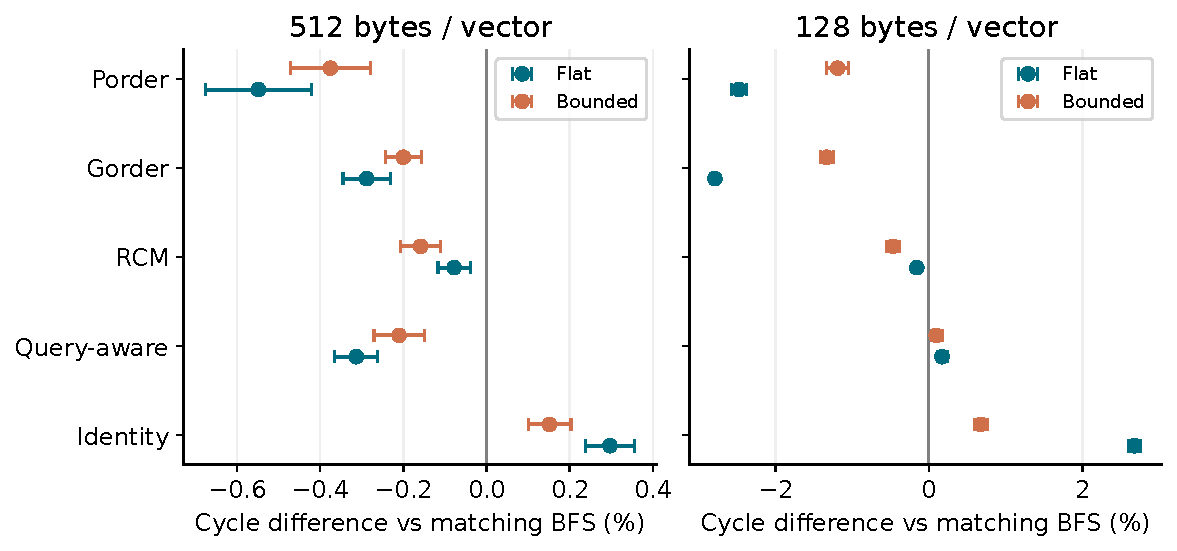
\includegraphics[width=\textwidth]{generated/followup_layouts.pdf}
\caption[Placement under flat and bounded replay]{Layout differences relative to matching BFS, with split-level 95\% intervals. The panels use different horizontal scales. The 128-byte representation is hypothetical.}\label{fig:followup-layouts}
\end{figure}

On the reference graph with expansion boundaries, Porder's cycle difference relative to BFS is \PorderBoundedFloat\% at 512 bytes, compared with \QABoundedFloat\% for the local query-aware heuristic. At 128 bytes, Gorder gives \GorderBoundedCompact\%, while the local heuristic gives \QABoundedCompact\%. These comparisons show why stronger baselines matter: a local heuristic's weak result does not exhaust the available placement improvements.

Porder and the local query-aware heuristic must not be treated as interchangeable implementations of one idea. Their training relationships and placement objectives differ. A weak result for the local heuristic cannot establish that query-guided placement fails in general. Conversely, a gain by a published method in this replay does not reproduce its authors' application-speedup claim. The complete numerical comparisons, including flat replay against identity, are retained in \texttt{results/followup\_summary.csv}.

\subsection{Ordering only the currently available vector reads}
Figure~\ref{fig:followup-schedules} and Table~\ref{tab:followup-schedules} compare address sorting and transaction round-robin with original-order bounded replay on the same placement. The comparison changes order alone: each phase contains exactly the same multiset of transactions. Saved cycles per original query put the relative effect beside an absolute service-time allowance before any scheduling overhead.

\begin{table}[htbp]\centering\small
\caption[Within-expansion request schedules]{Reference graph, ten paired splits. Each schedule is compared with original-order bounded replay of the same layout. Negative percentage differences and positive saved-cycle counts favour the schedule.}\label{tab:followup-schedules}
\resizebox{\textwidth}{!}{\begin{tabular}{lrrrr}
\toprule
Bytes & Layout & Schedule & $\Delta$ cycles (\%) & Saved cycles/query \\
\midrule
512 & BFS & Sorted & +0.19 [+0.13, +0.24] & -74.5 \\
512 & BFS & Round-robin & -14.58 [-14.64, -14.51] & +5802.4 \\
512 & Query-aware & Sorted & +1.79 [+1.75, +1.84] & -712.5 \\
512 & Query-aware & Round-robin & -14.20 [-14.25, -14.15] & +5640.2 \\
128 & BFS & Sorted & +0.17 [+0.12, +0.21] & -26.1 \\
128 & BFS & Round-robin & +3.43 [+3.31, +3.55] & -540.5 \\
128 & Query-aware & Sorted & +1.00 [+0.91, +1.09] & -157.7 \\
128 & Query-aware & Round-robin & +3.30 [+3.21, +3.40] & -521.6 \\
\bottomrule
\end{tabular}
}
\end{table}

\begin{figure}[htbp]\centering
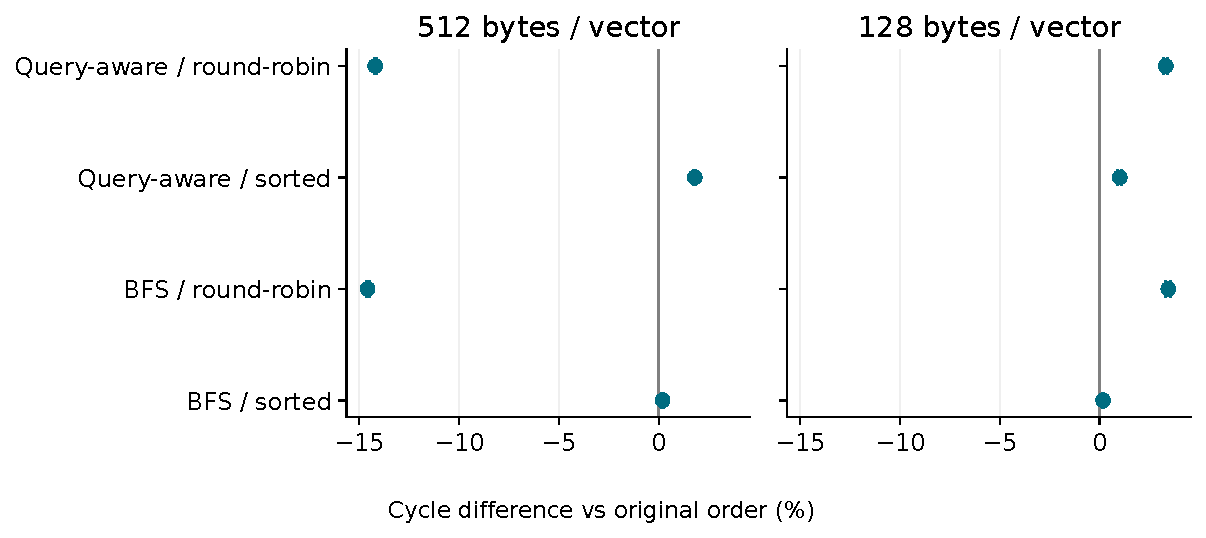
\includegraphics[width=\textwidth]{generated/followup_schedules.pdf}
\caption[When available-request schedules help or hurt]{Mean cycle differences and 95\% intervals on the reference graph. Both panels share the same scale. Every point compares a schedule with original-order bounded replay on the same layout; values left of zero favour the schedule.}\label{fig:followup-schedules}
\end{figure}

The two widths expose different amounts of logical work through a 64-transaction limit. Sixteen chunks belong to one 512-byte vector, but only four to a 128-byte vector. Round-robin exposes several vectors' chunks earlier instead of submitting every chunk of one vector first. This can improve the distribution of offered work, but can also disrupt useful row reuse. Sorting pursues nearby addresses and can have the opposite effect on bank diversity. Neither choice is automatically beneficial.

The per-query check uses the same reconstructed original-query service intervals. For BFS round-robin at 512 bytes, \RRFasterQueriesFloat\% of query records improve in each of the 19 graph/split cases. The within-case empirical 95th-percentile service difference ranges from \RRPtailRangeFloat\%. These are descriptive checks on sets of 200 queries; query IDs can recur between splits, and these records are not additional independent replications. They are service-time observations, not application latency guarantees.

\subsection{Explaining the scheduling contrast}
Four diagnostic replays add command recording to the first reference split's BFS original and round-robin streams at both widths. These repeats were selected after the pilot to explain its contrast; they are not independent statistical observations. They reproduce every original phase service interval and total timing exactly.

\begin{table}[htbp]\centering\small
\caption[Scheduling mechanism on the pilot split]{BFS, reference split one, bounded replay. ACT and PRE count row-opening and row-closing commands. ``No command'' counts controller cycles without a selected command. ``Banks'' is the mean number of distinct bank instances in full 64-request input windows wholly within one phase.}\label{tab:followup-mechanism}
\resizebox{\textwidth}{!}{\begin{tabular}{lrrrrrr}
\toprule
Bytes & Order & Cycles & ACT & PRE & No command & Banks \\
\midrule
512 & Original & 7825346 & 212732 & 113479 & 4267185 & 4.75 \\
512 & Round-robin & 6673884 & 347624 & 257071 & 2837829 & 15.07 \\
128 & Original & 3110725 & 197550 & 150156 & 1921043 & 14.10 \\
128 & Round-robin & 3214160 & 223114 & 174508 & 1974508 & 18.50 \\
\bottomrule
\end{tabular}
}
\end{table}

At 512 bytes, round-robin adds \RRCmdExtraFloat{} command-issue cycles but removes \RRNoCmdDeltaFloat{} cycles with no selected command, saving \RRStreamDeltaFloat{} cycles overall. Offered bank diversity increases from \RRBanksBeforeFloat{} to \RRBanksAfterFloat{} in the measured windows, while the classified row-hit fraction falls from \RRHitBeforeFloat{}\% to \RRHitAfterFloat{}\%. This is consistent with useful overlap outweighing additional row operations. At 128 bytes, the corresponding changes add \RRCmdExtraCompact{} command cycles and \RRNoCmdDeltaCompact{} no-command cycles, costing \RRStreamDeltaCompact{} cycles. Its original stream already offers \RRBanksBeforeCompact{} banks on average in those windows; round-robin raises that to \RRBanksAfterCompact{} without improving total service. These are within-width comparisons, because the two widths produce different numbers of full windows.

The accounting is exact, but it does not assign every no-command cycle to a particular DRAM timing rule. Phase completion waits, frontend availability, refresh and timing restrictions can contribute. Offered-bank diversity is an input statistic, not instantaneous controller occupancy. Even mean individual read latency falls in both cases; the slower 128-byte total therefore reinforces the need to measure completion of the whole workload. A proxy can explain part of a result without being an adequate optimisation target.

\subsection{Construction variation and preprocessing}
Tables~\ref{tab:followup-graphs} and \ref{tab:followup-schedule-graphs} retain all selected construction comparisons on matched splits one through three. They give means and observed ranges, without treating four selected graphs as a sampled population. The broader reference-graph estimate remains the ten-split interval reported above.

The boundaries can change a placement verdict. With graph seed 101, the local query-aware method loses to BFS at 128 bytes under bounded replay, although the earlier flat comparison favoured it. At 512 bytes, graph seed 101 on split two also reverses the small query-aware advantage. The earlier claim of improvement in every selected 512-byte case therefore applies specifically to flat replay. Gorder and Porder reduce total bounded service relative to BFS in all 19 cases at both widths. Round-robin retains its 512-byte improvement and 128-byte loss across all tested constructions on both evaluated placements.

\begin{table}[htbp]\centering\small
\caption[Bounded placement across graph constructions]{Cycle differences relative to BFS under bounded replay. Entries show means and observed ranges over three matched splits, all in percent.}\label{tab:followup-graphs}
\resizebox{\textwidth}{!}{\begin{tabular}{lrrrrr}
\toprule
Graph & Bytes & Query-aware & RCM & Gorder & Porder \\
\midrule
Reference & 512 & -0.26 [-0.30, -0.21] & -0.20 [-0.30, -0.13] & -0.24 [-0.28, -0.20] & -0.37 [-0.50, -0.23] \\
Reference & 128 & +0.06 [+0.01, +0.14] & -0.47 [-0.53, -0.34] & -1.30 [-1.34, -1.23] & -1.15 [-1.54, -0.79] \\
Seed 101 & 512 & -0.09 [-0.20, +0.02] & +0.06 [+0.03, +0.09] & -0.35 [-0.46, -0.30] & -0.37 [-0.56, -0.25] \\
Seed 101 & 128 & +0.24 [+0.16, +0.33] & -0.00 [-0.17, +0.09] & -1.10 [-1.17, -0.98] & -0.97 [-1.13, -0.85] \\
Seed 102 & 512 & -0.28 [-0.41, -0.20] & -0.12 [-0.23, -0.04] & -0.27 [-0.42, -0.19] & -0.53 [-0.62, -0.45] \\
Seed 102 & 128 & -0.52 [-0.67, -0.32] & -0.71 [-0.83, -0.62] & -1.89 [-1.98, -1.73] & -1.69 [-1.81, -1.63] \\
Shuffled 17 & 512 & -0.21 [-0.23, -0.17] & -0.17 [-0.20, -0.14] & -0.27 [-0.37, -0.20] & -0.39 [-0.65, -0.23] \\
Shuffled 17 & 128 & +0.42 [+0.19, +0.58] & +0.36 [+0.18, +0.50] & -1.05 [-1.14, -0.90] & -1.08 [-1.24, -0.89] \\
\bottomrule
\end{tabular}
}
\end{table}
\begin{table}[htbp]\centering\small
\caption[Scheduling across graph constructions]{Cycle differences relative to the same placement's original-order bounded replay. Entries show means and observed ranges over three matched splits, in percent. QA denotes the local query-aware placement.}\label{tab:followup-schedule-graphs}
\resizebox{\textwidth}{!}{\begin{tabular}{lrrrrr}
\toprule
Graph & Bytes & BFS sorted & BFS round-robin & QA sorted & QA round-robin \\
\midrule
Reference & 512 & +0.13 [+0.09, +0.21] & -14.56 [-14.71, -14.48] & +1.83 [+1.79, +1.85] & -14.19 [-14.31, -14.08] \\
Reference & 128 & +0.16 [+0.08, +0.21] & +3.43 [+3.33, +3.51] & +1.08 [+0.93, +1.22] & +3.30 [+3.06, +3.51] \\
Seed 101 & 512 & +0.17 [+0.10, +0.22] & -14.16 [-14.19, -14.09] & +1.70 [+1.68, +1.72] & -14.22 [-14.23, -14.20] \\
Seed 101 & 128 & +0.39 [+0.30, +0.50] & +3.59 [+3.28, +3.78] & +0.94 [+0.88, +1.01] & +3.18 [+2.86, +3.36] \\
Seed 102 & 512 & +0.33 [+0.26, +0.39] & -14.26 [-14.29, -14.22] & +1.67 [+1.56, +1.80] & -14.23 [-14.27, -14.14] \\
Seed 102 & 128 & +0.34 [+0.27, +0.39] & +3.71 [+3.45, +3.87] & +0.71 [+0.55, +0.95] & +3.19 [+3.07, +3.42] \\
Shuffled 17 & 512 & +0.44 [+0.39, +0.46] & -14.30 [-14.34, -14.27] & +1.80 [+1.73, +1.87] & -14.15 [-14.24, -14.03] \\
Shuffled 17 & 128 & +0.54 [+0.50, +0.59] & +3.66 [+3.59, +3.75] & +0.79 [+0.71, +0.89] & +3.18 [+2.99, +3.31] \\
\bottomrule
\end{tabular}
}
\end{table}

\begin{table}[htbp]\centering
\caption[Published-layout preprocessing]{Observed shared-host layout construction time across the 19 graph/split cases. Porder uses the adapted queue; graph loading, training searches and profile extraction are excluded. These are implementation cost observations, not isolated algorithm throughput benchmarks.}\label{tab:followup-cost}
\begin{tabular}{lrr}
\toprule
Layout & Mean (s) & Observed range (s) \\
\midrule
RCM & 0.094 & 0.082--0.114 \\
Gorder & 5.963 & 5.612--6.854 \\
Porder & 16.049 & 15.289--17.067 \\
\bottomrule
\end{tabular}

\end{table}
The scheduling matrix covers BFS and the local query-aware placement. It does not test every published-layout/schedule combination, so separate placement and scheduling gains must not be added to predict a combined result.

Published methods also require preprocessing (Table~\ref{tab:followup-cost}). Porder additionally requires a training profile. Round-robin needs candidate addresses and enough temporary state to keep track of chunks; sorting needs that state plus ordering work. The replay times charge neither schedule for those operations. A useful next implementation must measure them against the saved service cycles and account for cache or local-memory reuse. The evidence identifies conditional memory-service opportunities, rather than a free deployment gain.
